\subusecasebase{Condivisione della prenotazione}
\label{usecase:Condivisione della prenotazione}

\begin{figure}[h]
	\centering
	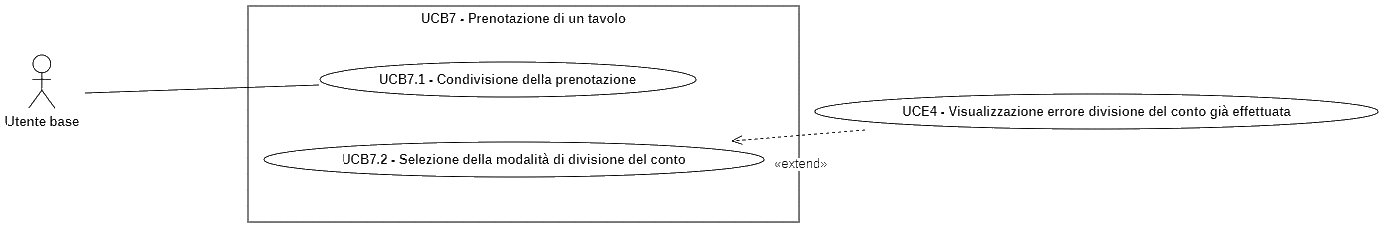
\includegraphics[width=0.99\textwidth]{./uml/UCB7.1-UCB7.2.png} 
	\caption{Condivisione della prenotazione}
	\label{fig:UCB9}
  \end{figure}

\begin{itemize}
	\item \textbf{Attore principale:} Utente base.

	\item \textbf{Precondizioni:}
	\begin{itemize}
		\item L'Utente base ha effettuato l'accesso al Sistema (vedi \autoref{usecase:Effettua accesso}).
		\item L'Utente base sta creando una prenotazione (vedi \autoref{usecase:Prenotazione di un tavolo}).
	\end{itemize}

	\item \textbf{Postcondizione:}
	      L'Utente base ha invitato gli altri commensali alla prenotazione.

	\item \textbf{Scenario principale:}
	      \begin{enumerate}
		      \item L'Utente base inserisce tutte le \textit{email} degli altri utenti che vuole invitare alla prenotazione;
		      \item Il Sistema collega gli utenti invitati alla prenotazione;
	      \end{enumerate}
\end{itemize}
